\documentclass[12pt]{article}

% Original packages
\usepackage{amsmath}
\usepackage{geometry}
\usepackage{algorithm}
\usepackage{algorithmic}
\usepackage{amsthm}
\usepackage{graphicx}
\usepackage{setspace}
\usepackage{enumitem}
\usepackage{tikz}
\usepackage{amsfonts}
\usepackage{amssymb}
\usepackage{pgfplots}
\usepackage{pgfplotstable}
\usepackage{booktabs}
\usepackage{caption}
\usepackage{subcaption}
\usepackage{float}
\usepackage{fancyhdr}
\usepackage{lastpage}

\usepackage{multirow}
\usepackage{booktabs} % For better-looking tables

\usepackage{afterpage}

\usepackage{listings}

\usepackage{tabularx}  % Add this to your preamble
\usepackage{booktabs} % For professional table lines

% Additional packages for hyperlinks and PDF features
\usepackage{hyperref}
\usepackage{bookmark}
\usepackage{xcolor}

% Configure hyperlinks
\hypersetup{
    colorlinks=true,
    linkcolor=black,
    filecolor=magenta,      
    urlcolor=cyan,
    pdftitle={Statistical Analysis of Activity-Travel Behavior},
    pdfauthor={Raswanth Prasath S V},
    pdfpagemode=UseOutlines,
    bookmarksnumbered=true
}

% Set page margins
\geometry{a4paper, margin=1in}

% Configure page style
\pagestyle{fancy}
\fancyhf{} % Clear default header/footer

% Define header style
\fancyhead[L]{\small Regression Based Models of Activity Frequency}
\fancyhead[R]{\small Project-2}

% Define footer style
\fancyfoot[L]{\small }
\fancyfoot[C]{\small }
\fancyfoot[R]{\small Page \thepage\ }

% Set header/footer line width
\renewcommand{\headrulewidth}{0.4pt}
\renewcommand{\footrulewidth}{0.4pt}

% Adjust header/footer margins
\setlength{\headheight}{15pt}

% Create a plain style for chapter/section first pages
\fancypagestyle{plain}{
    \fancyhf{} % Clear all header/footer fields
    \fancyfoot[L]{\small Raswanth Prasath S V}
    \fancyfoot[C]{\small}
    \fancyfoot[R]{\small Page \thepage\ of \pageref{LastPage}}
    \renewcommand{\headrulewidth}{0.4pt}
    \renewcommand{\footrulewidth}{0.4pt}
}


\begin{document}

% Remove page numbering for cover page
\pagenumbering{gobble}

% Remove headers/footers from cover page
\thispagestyle{empty}

% Cover page
\begin{center}
    \vspace*{1.5cm}
    
    \textbf{\Large Statistical Analysis of Activity-Travel}
    
    \textbf{\Large Behavior Characteristics}
    
    \vspace{6cm}
    
    \textbf{\Large CEE 598: Activity-Travel Behavior Modeling and Simulation}
    
    \vspace{6cm}
    
    \large{Raswanth Prasath S V}
    
    \vspace{0.5cm}
    
    \large{School of Sustainable Engineering and the Built Environment}
    
    \large{Arizona State University}
    
    \vspace{2cm}
    
    \large{Spring 2025}
    
    \vfill
    
\end{center}

% Start new page for TOC and lists
\newpage
\pagenumbering{roman}

% Table of Contents
\tableofcontents
\newpage

% List of Figures
\listoffigures

% List of Tables
\listoftables
\newpage

% Start main content with Arabic numbering
\pagenumbering{arabic}

% Main document content
\section{Introduction}

\par{This project aims to conducted a statistical analysis of travel behavior characteristics, examining how different demographic and socioeconomic factors influence various aspects of travel. The project examined five key aspects of travel behavior: activity patterns, trip purposes, transportation mode choices, time-of-day travel patterns, and activity durations for different purposes. Using statistical analysis and hypothesis testing, the revealed important differences in how various groups - such as workers vs. non-workers, older adults vs. others, and households with different income levels and car availability - interact with transportation systems. These insights can help inform transportation planning and policy decisions to better serve diverse community needs.}

\section{Data Preparation and Methodology}
This project uses data from the 2017 National Household Travel Survey (NHTS), obtained from \href{http://nhts.ornl.gov/}{http://nhts.ornl.gov/}. As the nation's authoritative source on daily travel patterns, the NHTS captures detailed information about how, why, when, and where people travel. The NHTS data structure consists of four interrelated files: The Household File, Person File, Trip File and the Vehicle File. 

The dataset was prepared by filtering the 2017 NHTS data to include only: Households in Arizona, New Mexico, Colorado, and Utah , Weekday trips (Monday through Friday), and Adults (18 years and older)


The analysis accounts for zero-trip makers to avoid selection bias. Trip counts were aggregated from individual trip records to the household level. Several binary indicator variables were created to represent categorical factors such as:
\begin{itemize}
    \item Home ownership (\texttt{home\_owner})
    \item Urban/rural status (\texttt{urban\_area})
    \item Income categories (\texttt{inc15}, \texttt{inc15\_35}, \texttt{inc35\_50}, \texttt{inc50\_75}, \texttt{inc75\_100}, \texttt{inc100p})
    \item Worker status (\texttt{worker1}, \texttt{worker2p})
    \item Travel behavior (\texttt{active\_traveler}, \texttt{car\_user})
    \item Internet usage (\texttt{daily\_web\_user})
\end{itemize}

Additional derived variables were created to capture more complex relationships:
\begin{itemize}
    \item Adult to household size ratio (\texttt{adult\_ratio})
    \item Vehicle to household size ratio (\texttt{veh\_per\_person})
    \item Logarithmic transformation of household size (\texttt{log\_hhsize})
    \item Interaction between high income and multiple workers (\texttt{inc\_worker\_interact})
    \item Interaction between high density and transit use (\texttt{density\_transit})
\end{itemize}


\section{Multiple Linear Regression Models of Total Household Weekday Trips}
Multiple linear regression models were estimated using the ordinary least squares (OLS) method. The general form of the model is:
\begin{equation}
Y = \beta_0 + \beta_1X_1 + \beta_2X_2 + ... + \beta_kX_k + \epsilon
\end{equation}
Where $Y$ represents total household weekday trips, $X_1$ through $X_k$ represent independent variables, $\beta_0$ through $\beta_k$ are coefficients to be estimated, and $\varepsilon$ is the error term.\\

Ten different model specifications were tested to identify the most appropriate representation of the relationship between household characteristics and trip generation. Model assessment was conducted using multiple criteria including statistical significance of parameters, goodness-of-fit measures, and elasticity calculations.


\subsection{Trip Generation Patterns}
Before developing the regression models, key patterns in the data were examined. Table \ref{tab:trip_stats} presents summary statistics for household trip counts and other key variables.

\begin{table}[h]
\centering
\caption{Summary Statistics of Key Variables}
\label{tab:trip_stats}
\begin{tabular}{lrrrr}
\toprule
Variable & Mean & Std. Dev. & Min & Max \\
\midrule
Household Trips & 6.17 & 4.80 & 0 & 35 \\
Household Size & 2.58 & 1.37 & 1 & 12 \\
Vehicles & 2.14 & 1.14 & 0 & 11 \\
Workers & 1.15 & 0.93 & 0 & 6 \\
\bottomrule
\end{tabular}
\end{table}


The average household in the sample makes approximately 6.17 trips on a typical weekday, with substantial variation (standard deviation of 4.80). About 8.5\% of households reported making zero trips on their assigned travel day.

\subsection{Model Specifications and Results}
\subsubsection{Model Development Strategy}
A systematic approach was employed to develop regression models for trip generation. Starting with basic socio-demographic variables, additional variables were incrementally added to improve model performance. Various forms of key variables (particularly household size and income) were tested to capture potential non-linear relationships.

\subsubsection{Model Specifications}
Ten different model specifications were tested:
\begin{itemize}
\item \textbf{Model 1}: Basic model with income categories only
\item \textbf{Model 2}: Income categories and household size
\item \textbf{Model 3}: Income categories, household size, and vehicle count
\item \textbf{Model 4}: Continuous income with quadratic term, household size, and vehicle count
\item \textbf{Model 5}: High/low income indicators, household size, worker status, and travel behavior
\item \textbf{Model 6}: Model 5 plus urban/rural status and lifecycle variables
\item \textbf{Model 7}: Log-transformed household size and other key variables
\item \textbf{Model 8}: Adult ratio and vehicle per person ratios
\item \textbf{Model 9}: Interaction terms between income, workers, and density
\item \textbf{Model 10}: Comprehensive model with built environment variables
\end{itemize}


\subsubsection{Model Comparison}
Table \ref{tab:model_comparison} presents a comparison of all models based on key performance metrics.

\begin{table}[h]
\centering
\caption{Comparison of Model Performance}
\label{tab:model_comparison}
\begin{tabular}{lrrr}
\toprule
Model & AIC & BIC & Adjusted $R^2$ \\
\midrule
Model 1 & 18358 & 18401 & 0.056 \\
Model 2 & 17989 & 18038 & 0.163 \\
Model 3 & 17978 & 18032 & 0.166 \\
Model 4 & 17971 & 18007 & 0.167 \\
Model 5 & 17918 & 17966 & 0.182 \\
Model 6 & 17902 & 17969 & 0.187 \\
Model 7 & 17872 & 17927 & 0.194 \\
Model 8 & 18126 & 18186 & 0.126 \\
Model 9 & 17918 & 17978 & 0.183 \\
Model 10 & 17872 & 17939 & 0.195 \\
\bottomrule
\end{tabular}
\end{table}

% Model 10 exhibited the best overall performance with the highest adjusted R2^2
% 2 (0.195) and among the lowest AIC values (17872). Model 7, which incorporated log-transformed household size, also performed well with identical AIC but a slightly lower adjusted R2^2
% 2.

% \subsection{Best Model Results}
% Table \ref{tab:best_model} presents the detailed results for the best-performing model (Model 10).
\begin{table}[h]
\centering
\caption{Regression Results for Best Model (Model 10)}
\label{tab:best_model}
\begin{tabular}{lrrrr}
\toprule
Variable & Coefficient & Std. Error & $t$-value & $p$-value \\
\midrule
Intercept & -0.042 & 0.368 & -0.11 & 0.909 \\
High Income ($\geq\$100,000$) & 0.519 & 0.206 & 2.51 & 0.012* \\
Low Income ($\leq\$15,000$) & -0.767 & 0.262 & -2.93 & 0.004** \\
$\log(\text{Household Size})$ & 4.806 & 0.279 & 17.24 & <0.001*** \\
Multiple Workers & 1.308 & 0.217 & 6.02 & <0.001*** \\
Active Traveler & 1.089 & 0.175 & 6.22 & <0.001*** \\
Daily Web User & 0.470 & 0.246 & 1.91 & 0.056 \\
High Density & 0.324 & 0.311 & 1.04 & 0.296 \\
Households per Population Density & -0.00003 & 0.00004 & -0.77 & 0.442 \\
Housing Type per Population Density & -0.00005 & 0.00004 & -1.14 & 0.254 \\
\bottomrule
\multicolumn{5}{l}{\textit{Significance codes: *** $p<0.001$, ** $p<0.01$, * $p<0.05$}}
\end{tabular}
\end{table}

The best model explains approximately 19.5\% of the variance in household trip generation (Adjusted RSquare
2 = 0.195). The F-statistic of 83.9 (p < 0.001) indicates that the model is statistically significant.

The most influential variables in the model are:
\begin{itemize}
    \item \textbf{Household size (log-transformed)}: Each unit increase in log-transformed household size is associated with approximately 4.8 additional trips per day, indicating strong economies of scale in household trip-making.
    \item \textbf{Multiple workers}: Households with two or more workers make about 1.3 more trips compared to households with zero or one worker.
    \item \textbf{Active travelers}: Households with members who engage in active transportation (walking or biking) make approximately 1.1 more total trips.
    \item \textbf{Income effects}: High-income households (income $\geq$ \$100,000) make about 0.5 more trips, while low-income households (income $\leq$ \$15,000) make about 0.8 fewer trips compared to middle-income households.
\end{itemize}

Interestingly, the density variables (HBPPOPDN and HTPPOPDN) are not statistically significant after controlling for other factors. This suggests that socio-demographic characteristics may be more important determinants of total trip generation than built environment characteristics.

\section{Residual Analysis of Household Trip Generation Models}

\subsection{Elasticity Analysis}
Elasticity measures the percentage change in the dependent variable (trips) for a one percent change in an independent variable. For continuous variables, elasticities were calculated using the formula:
\begin{equation}
E_{x_i} = \beta_i \cdot \frac{\bar{x_i}}{\bar{y}}
\end{equation}

Where:
\begin{itemize} 
    \item $E_{x_i}$: Elasticity of variable $x_i$
    \item $\beta_i$: Regression coefficient for variable $x_i$
    \item $\bar{x_i}$: Mean of the independent variable
    \item $\bar{y}$: Mean of the dependent variable (total household trips)
\end{itemize}
Table \ref{tab:elasticities} presents elasticities for key continuous variables in the best model.

\begin{table}[h]
\centering
\caption{Elasticities for Continuous Variables}
\label{tab:elasticities}
\begin{tabular}{lr}
\toprule
Variable & Elasticity \\
\midrule
$\log(\text{Household Size})$ & 0.796 \\
$\text{HBPPOPDN}$ & -0.017 \\
$\text{HTPPOPDN}$ & -0.019 \\
\bottomrule
\end{tabular}
\end{table}


The elasticity for log-transformed household size is 0.796, indicating that a 1\% increase in household size is associated with approximately a 0.80\% increase in trip generation. This suggests that household size is a strong determinant of trip-making behavior, though the relationship is less than proportional due to the logarithmic transformation.
For dummy variables, we can interpret the effect as the percentage change in trip generation when the variable changes from 0 to 1. These effects were calculated as:

\begin{equation}
E_{dummy} = \frac{\beta_{dummy}}{\bar{y}}
\end{equation}

Table \ref{tab:dummy_effects} presents these effects for key dummy variables.
\begin{table}[h]
\centering
\caption{Effects of Dummy Variables on Trip Generation}
\label{tab:dummy_effects}
\begin{tabular}{lr}
\toprule
Variable & Effect \\
\midrule
High Income ($\geq\$100,000$) & 0.080 \\
Low Income ($\leq\$15,000$) & -0.119 \\
Multiple Workers & 0.202 \\
Active Traveler & 0.168 \\
Daily Web User & 0.073 \\
\bottomrule
\end{tabular}
\end{table}

The presence of multiple workers in a household has the largest effect, with such households making about 20.2\% more trips compared to households with zero or one worker. Households with active travelers make about 16.8\% more trips, while high-income households make 8.0\% more trips and low-income households make 11.9\% fewer trips compared to middle-income households.

\subsubsection{Diagnostic Tests}
Several diagnostic tests were performed to assess model assumptions. Figure \ref{fig:residuals} shows the distribution of residuals.

\begin{figure}[H]
\centering
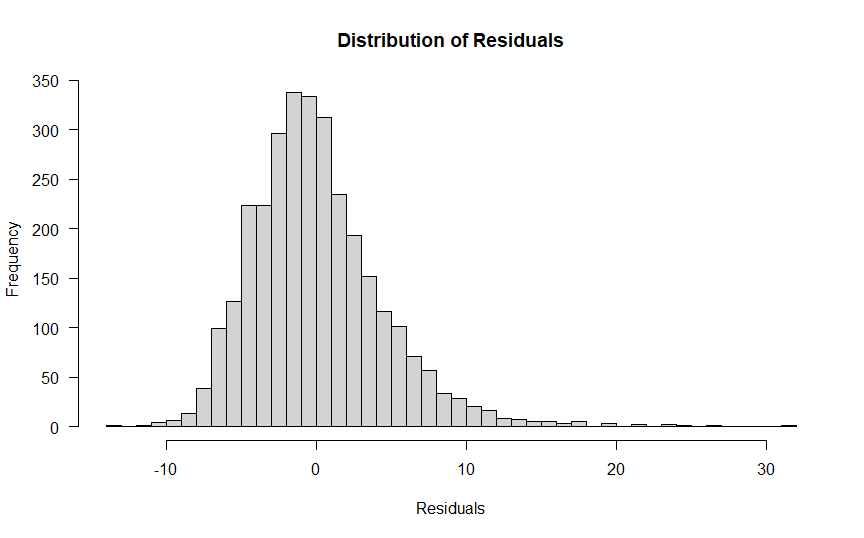
\includegraphics[width=0.7\textwidth]{media/Distribution of Residuals.png}
\caption{Distribution of Residuals}
\label{fig:residuals}
\end{figure}


Figure \ref{fig:residplot} shows the plot of residuals versus fitted values.
\begin{figure}[H]
\centering
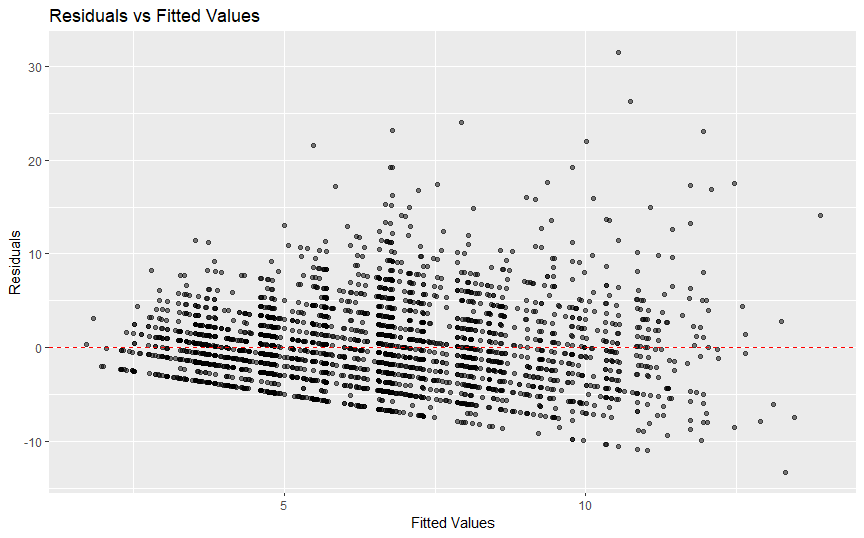
\includegraphics[width=0.7\textwidth]{media/Residuals vs. Fitted Values.png}
\caption{Residuals vs. Fitted Values}
\label{fig:residplot}
\end{figure}


% Figure \ref{fig:diagnostics} presents the four standard diagnostic plots for regression analysis.

% \begin{figure}[H]
% \centering
% \includegraphics[width=0.8\textwidth]{Image 3}
% \caption{Diagnostic Plots for Best Model}
% \label{fig:diagnostics}
% \end{figure}

The diagnostic plots reveal some issues with the model:
\begin{itemize}
\item \textbf{Non-normality}: The residuals show right-skewness, and the Q-Q plot indicates deviation from normality, particularly in the right tail. The Shapiro-Wilk test confirms significant non-normality (W = 0.9, p < 0.001).
\item \textbf{Heteroscedasticity}: The residuals vs. fitted plot shows a pattern of increasing variance with fitted values. The Breusch-Pagan test confirms significant heteroscedasticity (BP = 164, p < 0.001).

\item \textbf{Outliers}: Approximately 36 observations (about 1.2\% of the sample) have standardized residuals exceeding 3 standard deviations, indicating potential outliers.
\end{itemize}
\subsection{Multicollinearity Assessment}
Variance Inflation Factors (VIF) were calculated to assess multicollinearity among predictors. Table \ref{tab:vif} presents the VIF values for all variables in the best model.


\begin{table}[h]
\centering
\caption{Variance Inflation Factors for Best Model}
\label{tab:vif}
\begin{tabular}{lr}
\toprule
Variable & VIF \\
\midrule
High Income ($\geq\$100,000$) & 1.1 \\
Low Income ($\leq\$15,000$) & 1.1 \\
$\log(\text{Household Size})$ & 1.3 \\
Multiple Workers & 1.3 \\
Active Traveler & 1.0 \\
Daily Web User & 1.1 \\
High Density & 3.1 \\
Households per Population Density & 4.2 \\
Housing Type per Population Density & 2.8 \\
\bottomrule
\end{tabular}
\end{table}

Most variables have VIF values below 2, indicating minimal multicollinearity concerns. The density variables show moderate multicollinearity (VIF between 2.8 and 4.2), but these values are still below the commonly used threshold of 5-10 for problematic multicollinearity.



\section{References}
\begin{enumerate}
\item Federal Highway Administration. (2017). 2017 National Household Travel Survey. U.S. Department of Transportation, Washington, DC.
\item Kitamura, R., Mokhtarian, P. L., \& Laidet, L. (1997). A micro-analysis of land use and travel in five neighborhoods in the San Francisco Bay Area. Transportation, 24(2), 125-158.

\item Purvis, C. L., Iglesias, M., \& Eisen, V. A. (1996). Incorporating work trip accessibility in nonwork trip generation models in San Francisco Bay Area. Transportation Research Record, 1556(1), 37-45.
\end{enumerate}



% -------------------------------------



\vspace{-0.5cm}


\end{document}